% calendar year
\newcommand{\calYear}{2021}
% if each week is to have 7 tracking circles to fill in
% if no, just filled with more notes space
\newcommand{\trackers}{yes}

\documentclass{scrartcl}
\pagestyle{empty}

% made to fit Notability on iPad Air
\usepackage[paperwidth=11in,paperheight=7in]{geometry}

\usepackage[hidelinks]{hyperref}
\usepackage{tikz}
\usetikzlibrary{positioning, calendar, shapes, calc}
\usepackage{ifthen}
\usepackage[calc]{datetime2}

\newcount\CurrDateJul
\newcount\LastDateJul

% ifdate to match two conditions
% from https://tex.stackexchange.com/questions/140948/tikz-calendar-and-conditional-tests
\makeatletter
\def\pgfcalendar@matchesfalse{\global\let\ifpgfcalendar@matches\iffalse}
\def\pgfcalendar@matchestrue{\global\let\ifpgfcalendar@matches\iftrue}
\pgfcalendar@matchesfalse
\pgfqkeys{/pgf/calendar}{and/.code 2 args={%
    \begingroup
      \ifdate{#1}{\ifdate{#2}{\pgfcalendar@matchestrue}{}}{}%
    \endgroup
    \ifpgfcalendar@matches\pgfcalendarmatchestrue\pgfcalendar@matchesfalse\fi}}
\makeatother

% calendar starts on Monday of first week of year, possibly in December
% from https://tex.stackexchange.com/questions/469059/how-to-get-the-monday-of-a-years-first-week
\newcount\FirstDayCount
\newcount\YearCount
\newcommand\GetMondaysDate[1]
  {%
    \pgfcalendardatetojulian{#1-01-01}\FirstDayCount
    \pgfcalendarjuliantoweekday{\FirstDayCount}\FirstDayCount
    \YearCount=#1
    \advance\YearCount-1
    \ifcase\FirstDayCount
      \def\MondaysDateIs{#1-01-01}%
    \or % 1
      \edef\MondaysDateIs{\the\YearCount -12-31}%
    \or % 2
      \edef\MondaysDateIs{\the\YearCount -12-30}%
    \or % 3
      \edef\MondaysDateIs{\the\YearCount -12-29}%
    \or % 4
      \edef\MondaysDateIs{\the\YearCount -12-28}%
    \or % 5
      \edef\MondaysDateIs{\the\YearCount -12-27}%
    \or % 6
      \edef\MondaysDateIs{\the\YearCount -12-26}%
    \fi
  }

% month labels for weekly calendars
% show up on Monday and first of the month
\tikzstyle{mymonth label}=[
  execute before day scope={
  \ifdate{Monday}{
    \node[anchor= east,xshift=-2ex,yshift=2.25ex,rotate=90]{\tikzmonthtext};}{},
  \ifdate{and={day of month = 1}{Tuesday}}{
    \node[anchor= east,xshift=-2ex,yshift=2.25ex,rotate=90]{\tikzmonthtext};}{},
  \ifdate{and={day of month = 1}{Wednesday}}{
    \node[anchor= east,xshift=-2ex,yshift=2.25ex,rotate=90]{\tikzmonthtext};}{},
  \ifdate{and={day of month = 1}{Thursday}}{
    \node[anchor= east,xshift=-2ex+8cm,yshift=2.25ex+18cm,rotate=90]{\tikzmonthtext};}{},
  \ifdate{and={day of month = 1}{Friday}}{
    \node[anchor= east,xshift=-2ex+8cm,yshift=2.25ex+18cm,rotate=90]{\tikzmonthtext};}{},
  \ifdate{and={day of month = 1}{Saturday}}{
    \node[anchor= east,xshift=-2ex+8cm,yshift=2.25ex+18cm,rotate=90]{\tikzmonthtext};}{},
  \ifdate{and={day of month = 1}{Sunday}}{
    \node[anchor= east,xshift=-2ex+8cm,yshift=2.25ex+18cm,rotate=90]{\tikzmonthtext};}{}
  }
]

% day labels for monthly calendars
% based on https://tex.stackexchange.com/questions/10186/weekday-captions-with-the-tikz-library-calendar
% can set options with day heading =
\makeatletter%
\tikzoption{day headings}{\tikzstyle{day heading}=[#1]}
\tikzstyle{day heading}=[]
\tikzstyle{day letter headings}=[
    execute before day scope={ \ifdate{day of month=1}{%
      \pgfmathsetlength{\pgf@ya}{\tikz@lib@cal@yshift}%
      \pgfmathsetlength\pgf@xa{\tikz@lib@cal@xshift}%
      \pgftransformyshift{-\pgf@ya}
      \foreach \d/\l in {0/Monday,1/Tuesday,2/Wednesday,3/Thursday,4/Friday,5/Saturday,6/Sunday} {
        \pgf@xa=\d\pgf@xa%
        \pgftransformxshift{\pgf@xa}%
        \pgftransformyshift{1cm}%
        \node[every day,day heading]{\l};%
      }
    }{}%
  }%
]
% day labels for yearly calendar
\tikzstyle{dayyear letter headings}=[
    execute before day scope={ \ifdate{day of month=1}{%
      \pgfmathsetlength{\pgf@ya}{\tikz@lib@cal@yshift}%
      \pgfmathsetlength\pgf@xa{\tikz@lib@cal@xshift}%
      \pgftransformyshift{-\pgf@ya}
      \foreach \d/\l in {0/m,1/t,2/w,3/t,4/f,5/s,6/s} {
        \pgf@xa=\d\pgf@xa%
        \pgftransformxshift{\pgf@xa}%
        \pgftransformyshift{\pgf@ya}%
        \node[every day,day heading]{\textit{\l}};%
      }
    }{}%
  }%
]
\makeatother%

% make the monthly calendar
\newcommand{\monthcal}[1]{%
    \newgeometry{left=.25in, top=0in, right=.25in, bottom=0in}
    \begin{tikzpicture}
    % 1x1 matrix just for positioning
    \matrix [anchor=month\DTMfetchmonth{#1}-\calYear-\DTMfetchmonth{#1}-01.center] at (0,0)
    {
    \calendar (month\DTMfetchmonth{#1}) [
        dates=\calYear-\DTMfetchmonth{#1}-01 to \calYear-\DTMfetchmonth{#1}-last,
        week list,
        month yshift = 0em,
        day letter headings,
        day xshift = 7.5em,
        day yshift = 6.5em,
        execute at end day scope={
            % box around day
            \draw[gray, thin] ($(month\DTMfetchmonth{#1}-\%y0-\%m0-\%d0.north east)+(-2.735,-2.35)$) rectangle ($(month\DTMfetchmonth{#1}-\%y0-\%m0-\%d0.north east)+(.15,.15)$);
            % dot paper for notes
            \ifdate{day of month=1}{
                \foreach \x in {3.5,4,...,8}
                \foreach \y in {-14.5,-14,...,1}
                {
                \fill[black] ($(month\DTMfetchmonth{#1}-\calYear-\DTMfetchmonth{#1}-01.north east)+(15-\pgfcalendarcurrentweekday*2.9+\x,\y)$) circle (.5pt);
                }
                \foreach \x in {4,4.5,...,7.5}
                {
                \fill[white] ($(month\DTMfetchmonth{#1}-\calYear-\DTMfetchmonth{#1}-01.north east)+(15-\pgfcalendarcurrentweekday*2.9+\x,0.5)$) circle (.5pt);
                }
                \node[text=black,anchor=center] at ($(month\DTMfetchmonth{#1}-\calYear-\DTMfetchmonth{#1}-01.north east)+(15-\pgfcalendarcurrentweekday*2.9+5.75,0.5)$) {\hyperlink{year}{\sffamily\bfseries \Huge \pgfcalendarmonthname{\DTMfetchmonth{#1}}}};
            }{} % end if first day of month
        }, % end end day scope
        day text={\hyperlink{myweek-\%y0-\%m0-\%d0}{\hypertarget{\pgfcalendarsuggestedname}{\%d-}}}
    ]
    if (weekend) [gray];\\
    };
    \end{tikzpicture}
    \restoregeometry
}

\begin{document}

\GetMondaysDate{\calYear}
\DTMsavedate{FirstDate}{\MondaysDateIs}

% blank page for yearly notes, goals
\begin{center}
    \hypertarget{goals}{\hyperlink{year}{\Huge\sffamily\bfseries \calYear}}
\end{center}

% yearly calendar
\newpage
\newgeometry{margin=.5in, bottom=0in}
\hypertarget{year}{}
\begin{center}
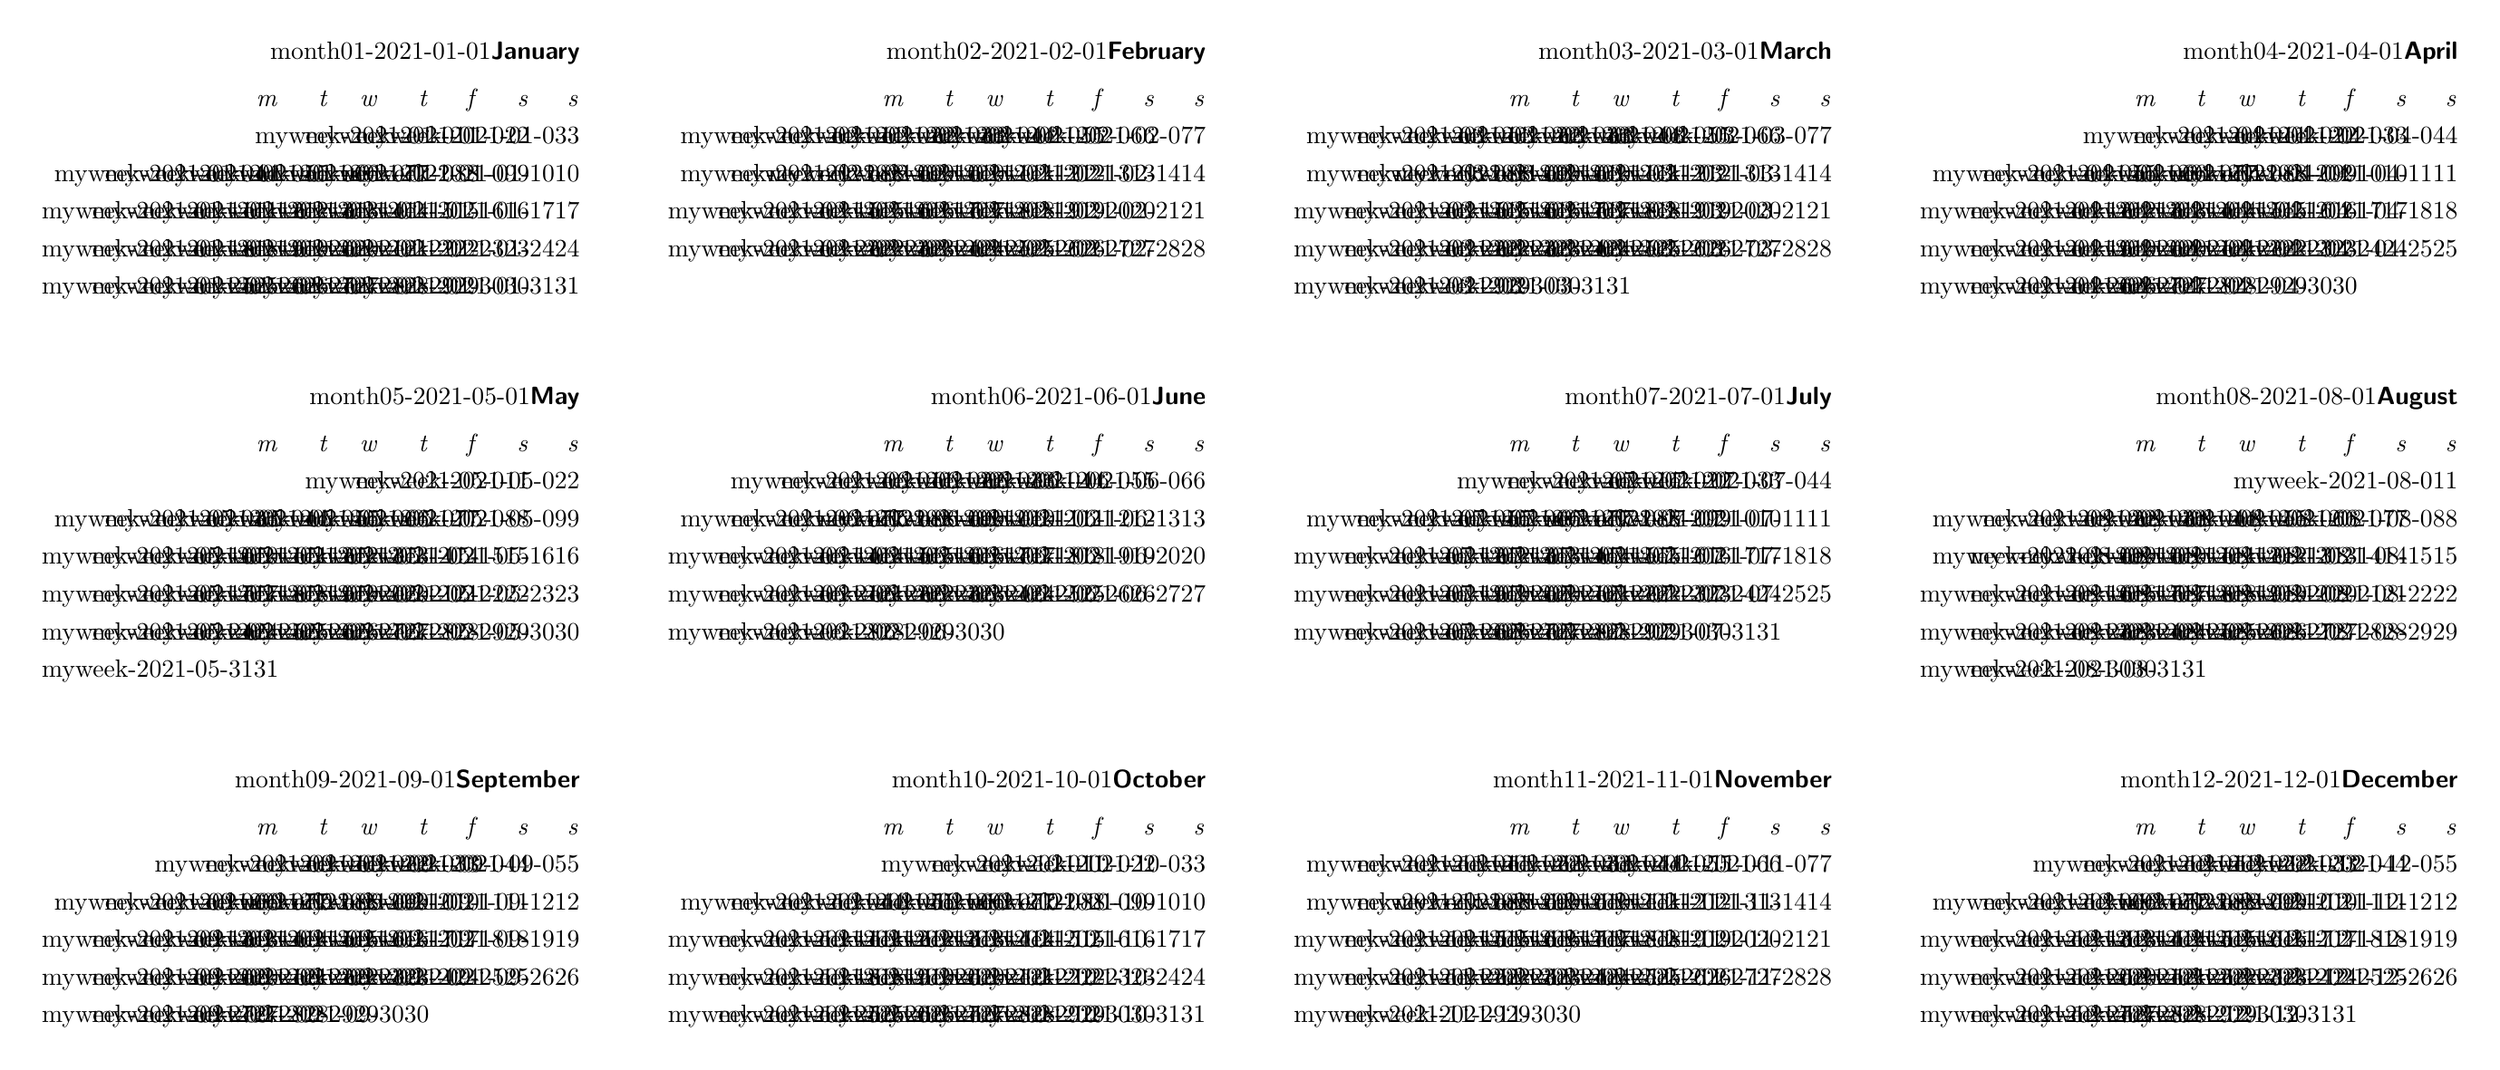
\begin{tikzpicture}[
    every calendar/.style={
        week list,
        month label above right,
        dayyear letter headings,
        day xshift = 2em,
        day yshift = 1.5em,
        day text={\hyperlink{myweek-\%y0-\%m0-\%d0}{\%d-}},
        month text={\hyperlink{month\%m0-\calYear-\%m0-01}{\sffamily\bfseries\%mt}}
    }]
    \matrix[column sep=1cm, row sep=1cm] {
        \calendar[dates=\calYear-01-01 to \calYear-01-last]; &
        \calendar[dates=\calYear-02-01 to \calYear-02-last]; &
        \calendar[dates=\calYear-03-01 to \calYear-03-last]; &
        \calendar[dates=\calYear-04-01 to \calYear-04-last]; \\
        \calendar[dates=\calYear-05-01 to \calYear-05-last]; &
        \calendar[dates=\calYear-06-01 to \calYear-06-last]; &
        \calendar[dates=\calYear-07-01 to \calYear-07-last]; &
        \calendar[dates=\calYear-08-01 to \calYear-08-last]; \\
        \calendar[dates=\calYear-09-01 to \calYear-09-last]; &
        \calendar[dates=\calYear-10-01 to \calYear-10-last]; &
        \calendar[dates=\calYear-11-01 to \calYear-11-last]; &
        \calendar[dates=\calYear-12-01 to \calYear-12-last]; \\
    };
\end{tikzpicture}
\end{center}
\restoregeometry

% iterate over all the weeks in the year
\newpage
\foreach \days in {0, 7, ..., 364}{

    % first and last day of week
    \DTMsaveddateoffsettojulianday{FirstDate}{\days}{\CurrDateJul}
    \DTMsavejulianday{CurrDate}{\CurrDateJul}
    \DTMsaveddateoffsettojulianday{CurrDate}{6}{\LastDateJul}
    \DTMsavejulianday{LastDate}{\LastDateJul}

    % if a new month starts this week, first put monthly calendar
    \DTMifdate{LastDate}{
        between=\DTMfetchyear{LastDate}-\DTMfetchmonth{LastDate}-01 and \DTMfetchyear{LastDate}-\DTMfetchmonth{LastDate}-07
    }{\monthcal{LastDate}}{}

    % make weekly calendar
    \newgeometry{left=.25in, top =.35in, bottom=0in, right=0in}
    \begin{tikzpicture}
    \tikzstyle{every day}=[anchor=base west]

    \calendar(myweek)[
        day list downward,
        mymonth label,
        month text={\hyperlink{month\DTMfetchmonth{CurrDate}-\%y0-\%m0-\%d0}{{\sffamily\bfseries \Huge \%mt}}},
        day text={\ifdate{Saturday}{\hypertarget{\pgfcalendarsuggestedname}{\%d-/}}{\hypertarget{\pgfcalendarsuggestedname}{\hyperlink{month\DTMfetchmonth{CurrDate}-\%y0-\%m0-\%d0}{\%d-}}}},
        month yshift = 0pt,
        day yshift = 6cm,
        execute at begin day scope=
        { % move Thurs-Sun to second column
            \ifdate{Thursday}{\pgftransformyshift{18cm}\pgftransformxshift{8cm}}{},
            \ifdate{Friday}{\pgftransformyshift{18cm}\pgftransformxshift{8cm}}{},
            \ifdate{Saturday}{\pgftransformyshift{18cm}\pgftransformxshift{8cm}}{},
            \ifdate{Sunday}{\pgftransformyshift{24cm}\pgftransformxshift{8.6cm}}{}
        },
        dates=\DTMusedate{CurrDate} to \DTMusedate{LastDate}, at={(1,22)}
    ];

    % dot paper for notes
    \foreach \x in {13.5, 14, ..., 21}
    \foreach \y in {-5, -4.5, ..., 7}
    {
        \fill (\x+5,\y+15.5) circle (.5pt);
    }
    \foreach \x in {16.5, 17, ..., 18}
    {
        \fill[white] (\x+5,6.5+15.5) circle (.5pt);
    }

    \node at (17.25+5,6.5+15.5) {{\sffamily\bfseries \Huge Notes}};

    % circle trackers for weekly tracking
    \ifthenelse{\equal{\trackers}{yes}}{%
        \foreach \x in {14.75, 15.75, 19, 20}
        {
            \node[draw, circle, minimum size=.99cm] at (\x+5,-6.5+15.5) {};
            \node[draw, circle, minimum size=.99cm] at (\x+5,-8.2+15.5) {};
        }
        \foreach \x in {14.25, 15.25, 16.25, 18.5, 19.5, 20.5}
        {
            \node[draw, circle, minimum size=.99cm] at (\x+5,-7.35+15.5) {};
        }
        \foreach \y/\l in {-6.25/P, -6.6/R, -6.95/O, -7.30/G, -7.65/R, -8/E, -8.35/S, -8.7/S}
        {
            \node at (17.375+5,\y+.07+15.5) {\hyperlink{goals}{\sffamily\bfseries \l}};
        }
    }{% if no trackers continue dots
        \foreach \x in {13.5, 14, ..., 21}
        \foreach \y in {-9, -8.5, ..., -5.5}
        {
            \fill (\x+5,\y+15.5) circle (.5pt);
        }
    } % end trackers

    \end{tikzpicture}
    \restoregeometry
 }

\end{document}
